
Loopy Belief Propagation~\cite{Murphy99loopybelief} (LBP) is an approximate inference algorithm
used in graphical models with cycles. In its essence, LBP is a sum-product message passing algorithm
where nodes exchange messages with their immediate neighbors and apply some computations to the messages
received.

LBP is an algorithm that maps very well to the graph based model of LM. In its
original form, the belief values of nodes are computed by synchronous iterations.
LBP offers more concurrency when belief values are computed asynchronously
leading to faster convergence. For this, every node keeps track of all messages
sent/received and recomputes the belief using partial information from neighbor
nodes. It is then possible to prioritize the computation of beliefs when a
neighbor's belief changes significantly.

The asynchronous approach proves to be a nice improvement over the synchronous
version. Still, it is possible to do even better. Gonzalez et
al~\cite{Gonzalez+al:aistats09paraml} developed an optimal algorithm to compute
this algorithm by first building a tree and then updating the beliefs of each
node twice, first from the leaves to the root and then from the root to the
leaves. The root of this tree is the node with the highest priority (based on
belief) while the other nodes in the tree must have a non-zero priority.
Note that the priorities are updated whenever a neighbor updates their belief.
These \emph{splash trees} are built iteratively until we reach convergence.

\begin{figure}[h!]
   \begin{center}
      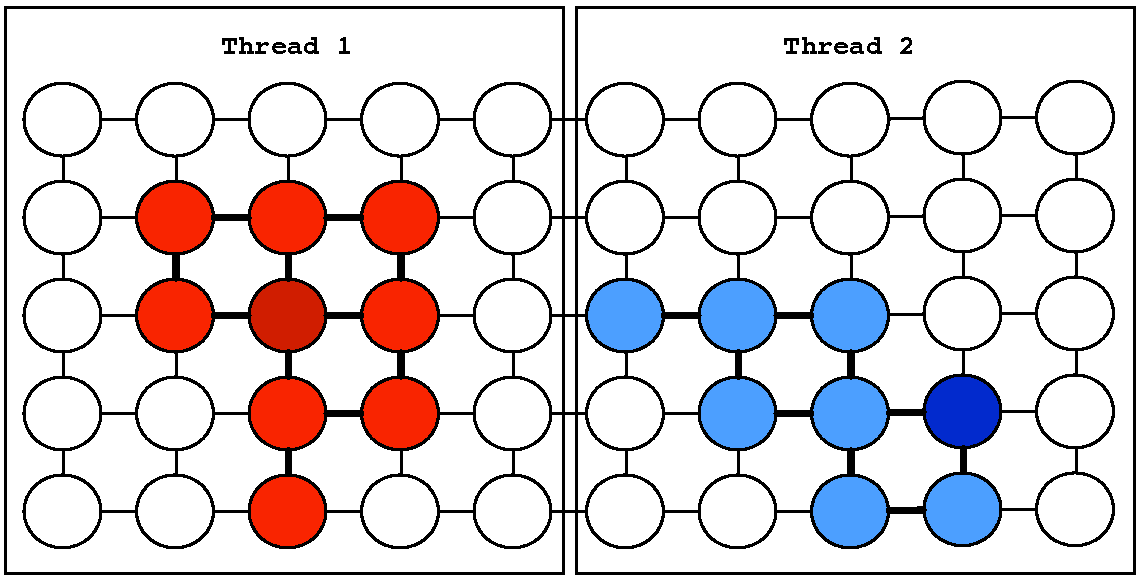
\includegraphics[width=6.5cm]{figures/splash_bp}
   \end{center}
   \caption{Single Source Shortest Path program code.}
   \label{splash_bp}
\end{figure}


The code for Splash Belief Propagation~(SBP) in Fig.~\ref{code:sbp} presents the
coordination code for LBP.  Please note that we just appended the code in
Fig.~\ref{code:sbp} to a working but unoptimized version of the algorithm, every
other logical rule remains the same. We add new logical ruels that coordinate
the creation and execution of the splash trees:

\begin{description}
   \item[Tree building]: Each node has a \texttt{waiting} fact that is used to
   start the tree building process. When the highest priority is picked, a token
   is created that will navigate through the tree. Note that in the rule located
   in lines 13-20, newly added nodes to the tree must have a positive priority
   (due to new belief updates) and must be residing in the same thread.
   We want the tree to be kept in the same thread in order to maximize
   parallelism with 1 tree per thread.
   \item[First phase]: In the third rule (lines 10-11), when the number of nodes
   of the tree reaches a certain limit, a 
   \texttt{first-phase} is generated in order to update the beliefs of all nodes
   in the tree, starting from the leaves and ending at the root
   As the nodes are updated, an \texttt{update} fact is derived to update
   the belief values (line 34).
   \item[Second phase]: In the second phase, the computation of beliefs is
   performed from the root to the leaves and the belief values are updated a
   second time (line 41).
\end{description}

When we have several threads, every thread will generate their own trees by
taking into account the highest priority node in their own queues. This is the
reason we use \texttt{set-static} in line 1 to force all nodes to remain in the
original threads.

\begin{figure}[h!]
\scriptsize\begin{Verbatim}[numbers=left,commandchars=*\{\}]
*underline{set-static(A)}. // all nodes are static.

// TREE BUILDING
// continue tree
waiting(A), token(A, All, Next) -o token(A, All, Next).
// start tree
waiting(A), *underline{@priority(A, A, P)}, P > 0.0
   -o token(A, [A], [A]).
// end tree building
token(A, All, Next), length(All) > maxnodes
   -o first-phase(A, All, reverse(All)).
// expand tree
token(A, All, [A | Next])
   -o [collect => L | Side | !edge(A, L, Side),
         0 = count(All, L),
         0 = count(Next, L),
         *underline{priority(A, L, P)}, P > 0.0,
         *underline{cpu-id(A, L, Id1)},
         *underline{cpu-id(A, A, Id2)}, Id1 = Id2 |
         send-token(A, All, Next ++ L)].

send-token(A, All, [])
   -o first-phase(A, All, reverse(All)).
send-token(A, All, [B | Next])
   -o *underline{schedule-next(B)},
      token(B, All ++ [B], [B | Next]).

// FIRST PHASE
first-phase(A, [A], [A]) -o second-phase(A, [], A).
first-phase(A, [A, B | Next], [A])
   -o update(A), *underline{schedule-next(B)},
      second-phase(B, [B | Next], A).
first-phase(A, All, [A, B | Next])
   -o update(A), *underline{schedule-next(B)},
      first-phase(B, All, [B | Next]).

// SECOND PHASE
second-phase(A, [], _)
   -o *underline{set-priority(A, 0.0)}, waiting(A), update(A).
second-phase(A, [A], Back)
   -o update(A), waiting(Back),
      waiting(A), *underline{set-priority(A, 0.0)}.
second-phase(A, [A, B | Next], Back)
   -o update(A), waiting(Back), *underline{schedule-next(B)},
      second-phase(B, [B | Next], A).
\end{Verbatim}
  \caption{Coordination code for the Splash Belief Propagation program.}
  \label{code:sbp}
\end{figure}
\normalsize

In this program, coordination assumes a far more important role than we have
seen before. Coordination rules fully drive the behavior of the algorithm and
although the final result of the algorithm is identical to the original
algorithm (minus probabilitistic errors), SBP works in a very different way.
A system that also implements SBP is
GraphLab~\cite{GraphLab2010}, a C++ framework for writing machine algorithms.
GraphLab provides the splash scheduler for these types of inferences as part of
the framework. This particular scheduler is around 350 lines of complicated C++ code.
With our coordination facts, it is possible to create fairly complicated coordination
patterns with only 12 simple logical rules.
